\subsection{Overview}
DREAM will be used by thousands of users each day, with different needs, and located all over the Telangana region. To achieve this result and to respect all the requirements stated in the RASD, DREAM will be developed as a distributed application with clients and servers. The client will only show the graphical interface to the end-user, while the back-end will execute and support all the business logic operations. 
\begin{figure}[hbt!]
\centering
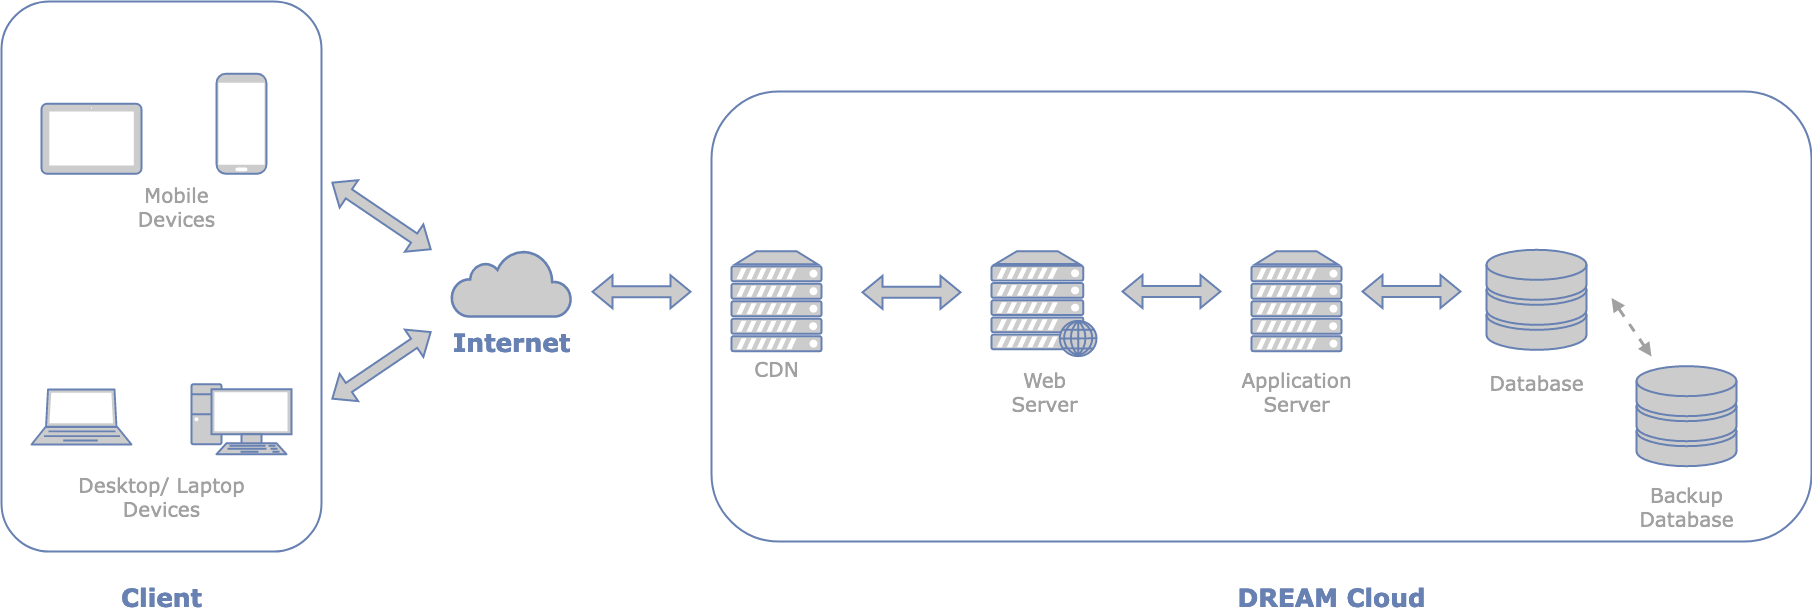
\includegraphics[width=\textwidth]{../images_diagrams/dd/highlevel_arch.png}
\caption{High-Level 5-tier Architecture.}
\label{fig:highLevelArch}
\end{figure}

\noindent
Since the application must be reliable and flexible enough in handling the growth of the user base, a cloud-based architecture is suitable for this task. In particular, DREAM Cloud is a 3-tier architecture with a web server, an application server, and a storage server (DBMS). To enable the system to always work in ideal conditions, a load balancer routes all the requests to different application servers. If necessary, new instances of the servers should be created and used to balance the computational load. An additional tier is then placed between the user and the DREAM Cloud: a Content Delivery Network. The CDN will relieve some load from the system and improve performances in serving static contents. Overall, the resulting application will have five tiers. Lastly, given the importance of the historical data kept inside the database, a backup system will frequently clone the data on a different server, possibly located in a different availability zone.

%\clearpage
\subsection{Component View}

The following diagrams will depict the internal structure of the DREAM system, demonstrating the components and interfaces that facilitate communication between them. The architecture consists of three different parts:
\begin{enumerate}
	\item the Agro-Farmer mobile web application which will be used by farmers and agronomists
	\item the Policy desktop web application used by policy makers
	\item the DREAM cloud that hosts the backend for all the previously introduced functionalities
\end{enumerate}
An additional element is presented for completeness: the Google Maps API is utilized by the mobile application to provide live turn-by-turn nagivation assistance. For simplicity, these three parts will be presented at different levels of abstraction, starting from the highest level, shown in Figure \ref{fig:highLevelComp}.\\

\begin{figure}[hbt!]
\centering
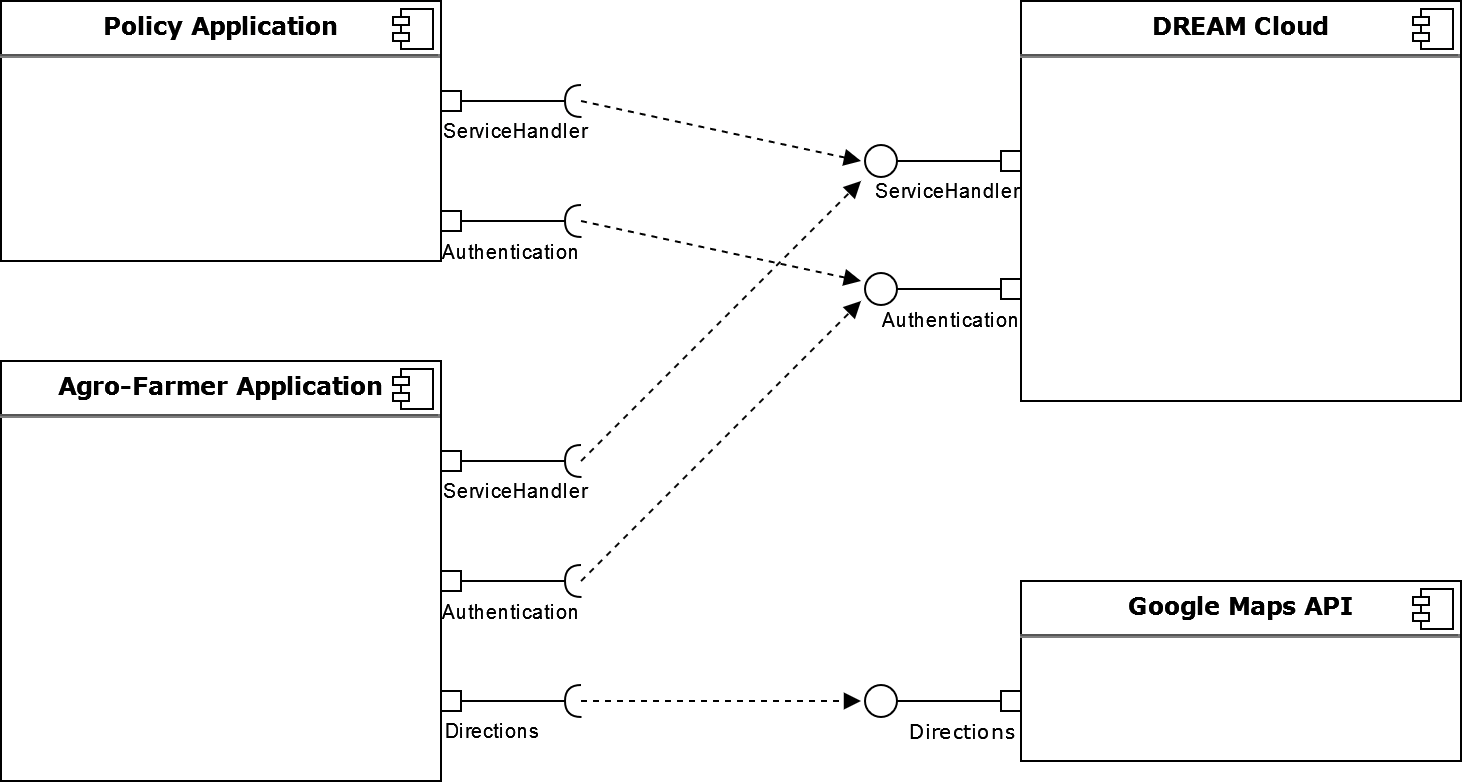
\includegraphics[width=\textwidth]{../images_diagrams/dd/high_level_cloud.png}
\caption{High-Level Component View.}
\label{fig:highLevelComp}
\end{figure}

\subsubsection{DREAM Cloud Component} \label{sect:cloudComponent}

\begin{figure}[hbt!]
\centering
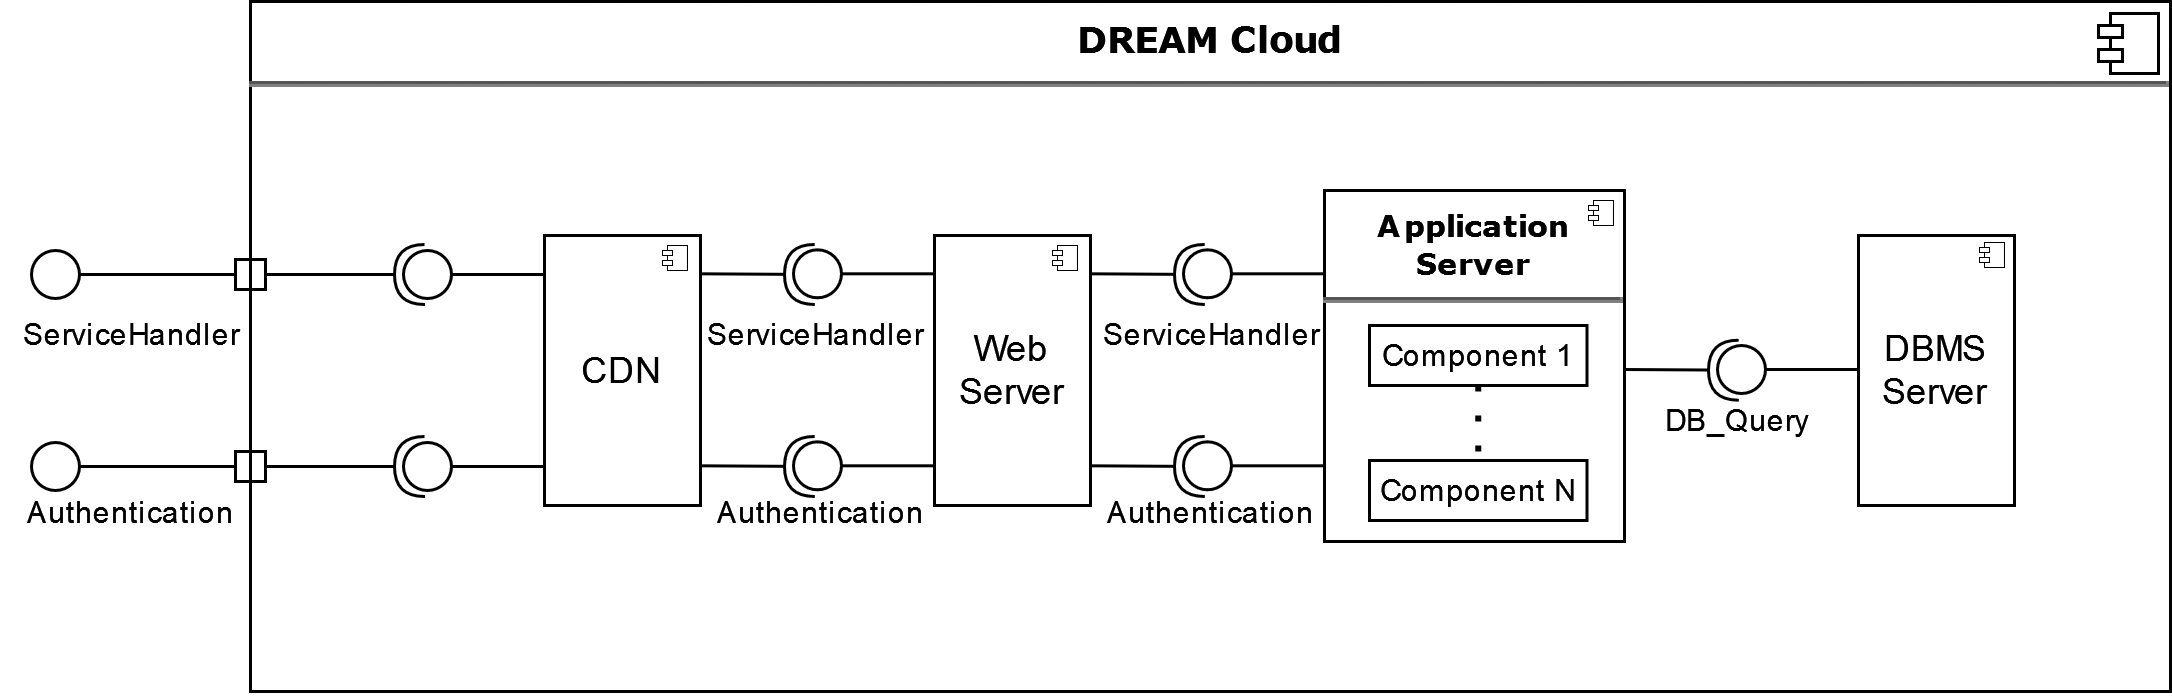
\includegraphics[width=\textwidth]{../images_diagrams/dd/component_only_cloud.png}
\caption{DREAM Cloud Component View.}
\label{fig:CloudOnlyComp}
\end{figure}

The cloud architecture illustrated in Figure \ref{fig:CloudOnlyComp} is based on the following components:
\begin{itemize}
	\item a CDN is implemented as the first component to improve the availability, performance, and redundancy of the entire system
	\item the Web Server is used to accept the HTTP requests and send HTTP responses. It provides static data as well as dynamic data obtained by the application server.
	\item the Application Server is the main component at this granularity. It contains about 15 smaller components that implement the business logic of the system. The dynamic content of the application is generated here.
	\item the DBMS server is responsible for the storage of data inside a database
\end{itemize}
Aside from the Application Server, all the others can be implemented using Commercial off-the-shelf products. \\

\subsubsection{Application Server Component}

The Figure \ref{fig:ApplicationServerOnlyComp} describes the application server and its components with the highest level of detail, as developers will have to implement the business logic themselves.\\

\begin{figure}[hbt!]
\centering
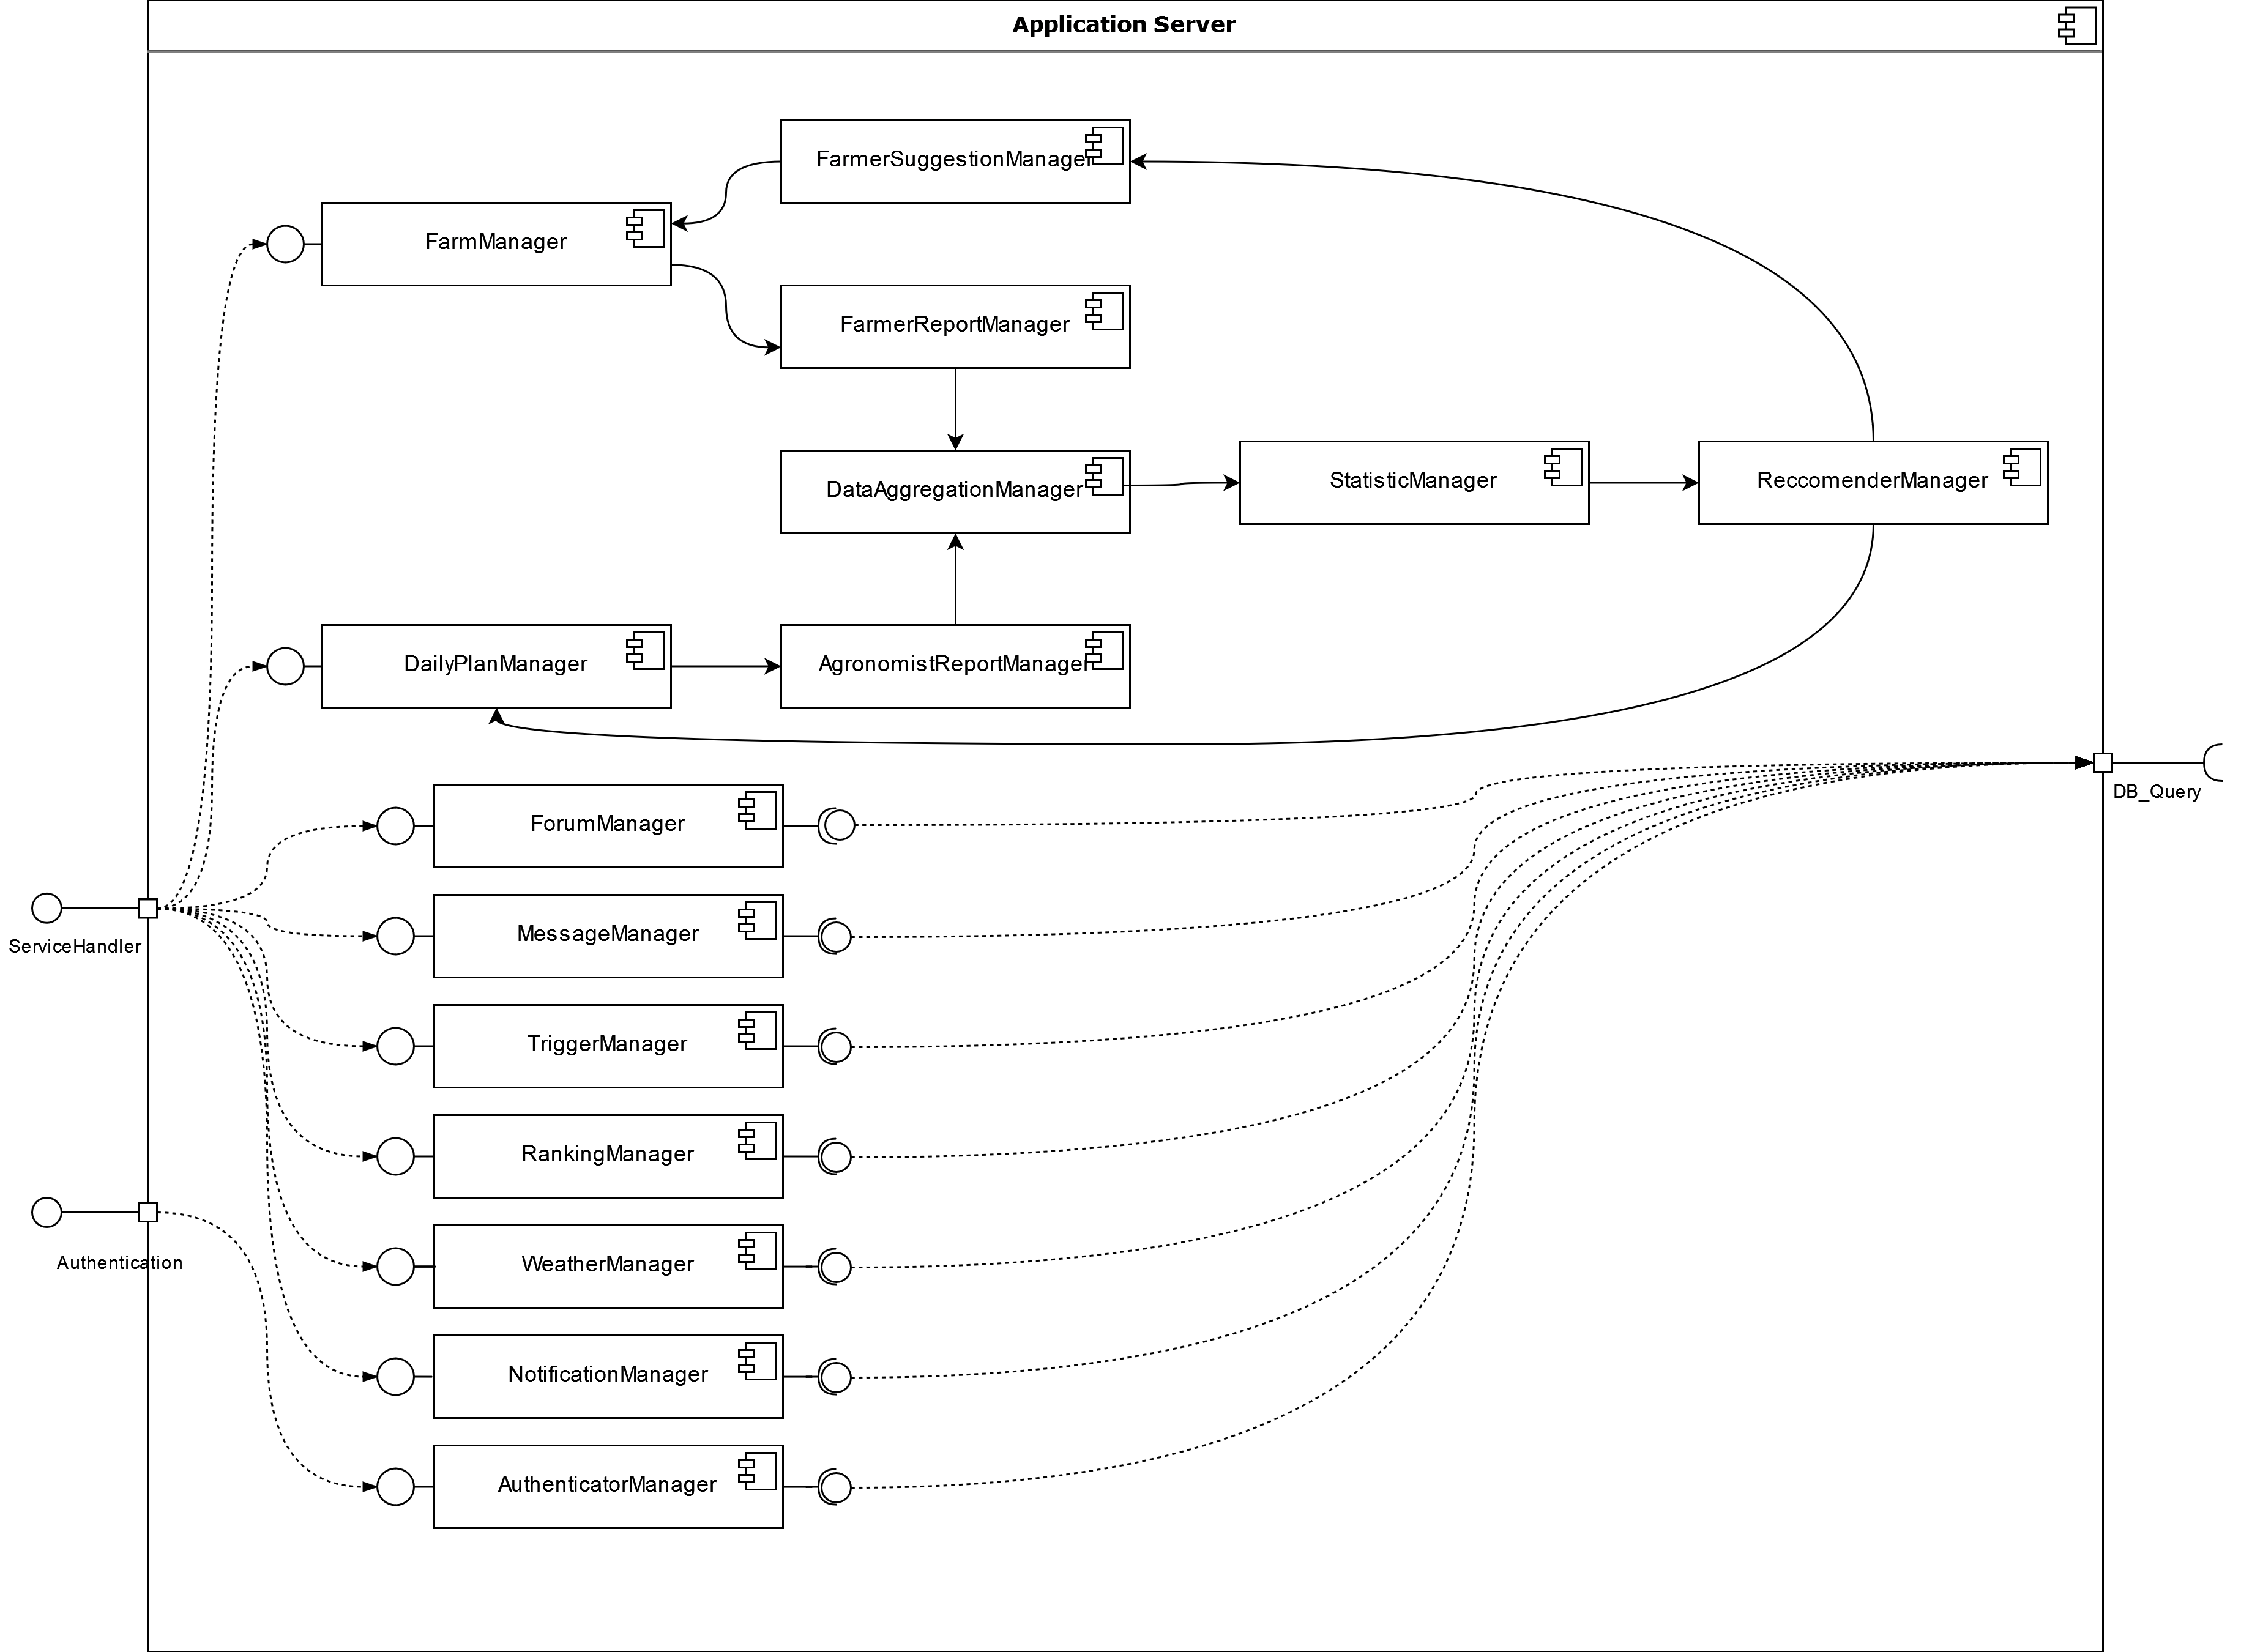
\includegraphics[width=\textwidth]{../images_diagrams/dd/component_only_application.png}
\caption{Application Server Component View.}
\label{fig:ApplicationServerOnlyComp}
\end{figure}

\noindent
The main components in the application server, providing all the business logic in DREAM, are:

\begin{itemize}
	\item The \textbf{AuthenticationManager} is responsible for the login, registration, and logout operation. It allows the users to use their credentials to get access to the application. It is also in charge of the password reset procedure.
	\item The \textbf{ForumManager} manages the Farmer Forum with the creation, deletion, and edits of posts and threads. 
	\item The \textbf{FarmManager} handles the "MyFarm" section in the mobile application, providing the farmer with all the information about their farm and fields.
	\item The \textbf{FarmerReportManager} is in charge of collecting the production data and other information about the yields from the farmer and storing everything inside the database.
	\item The \textbf{AgronomistReportManager} is in charge of collecting the production data, a score, and other information about the yields from the agronomist and storing everything inside the database.
	\item The \textbf{DataAggregationManager} is responsible for aggregating data and information obtained from the reports.
	\item The \textbf{StatisticsManager} manages the calculation of various statistics based on historical data.
	\item The \textbf{RecommenderManager} generates suggestions for farmers and agronomists, based on the previously calculated statistics.
	\item The \textbf{FarmerSuggestionManager} provides suggestions about the production, such as which plant species to plant or the fertilizers to use, to the farmers.
	\item The \textbf{DailyPlanManager} is responsible for the creation, edit, and confirmation of the daily plans.
	\item The \textbf{MessageManager} handles the communication between farmers and agronomists. It collects the message from the sender and forwards it to the recipient.
	\item The \textbf{NotificationManager} module is in charge of sending notifications to users. It is used on different occasions, such as when an agronomist receives a new message from a farmer or when there is a new thread in the Farmer Forum.
	\item The \textbf{TriggerManager} handles the creation, edit, and deletion of triggers by the policy makers. It creates a trigger at the database level, whenever possible, and executes a check for each trigger each time new data is provided through the reports.
	\item The \textbf{RankingManager} is responsible for the creation and update of farmer rankings based on the provided data and calculated statistics.
	\item The \textbf{WeatherManager} collects and provides data about the weather to farmers and agronomists.
\end{itemize}

\subsection{Deployment View}
\begin{figure}[hbt!]
\centering
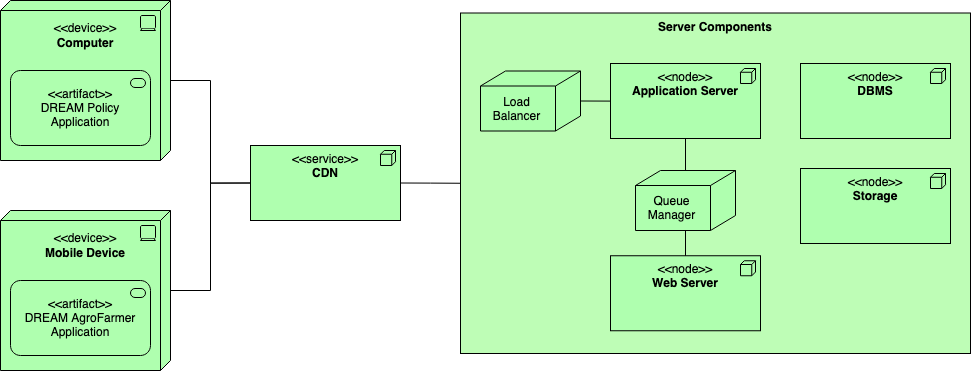
\includegraphics[width=\textwidth]{../images_diagrams/dd/highlevel_deployment.png}
\caption{High-Level Deployment View.}
\label{fig:highLevelDeploy}
\end{figure}

\begin{flushleft}
The main components in the deployment view in Figure \ref{fig:highLevelDeploy} are the client devices and the cloud platform. Policy makers will access the DREAM Policy Application via a computer device whereas agronomists and farmers will access the DREAM AgroFarmer Application via a mobile device. The CDN is represented as an external service. Then, the server components of the DREAM cloud include the application server, the web server, the database server, and the storage server. Within the cloud platform there is also a load balancer.
\end{flushleft}


\subsection{Runtime View}
You can use sequence diagrams to describe the way components interact
to accomplish specific tasks typically related to your use cases
\subsection{Component Interfaces}
This diagram shows the components of the application server with the main accessible methods.

\begin{figure}[hbt!]
\centering
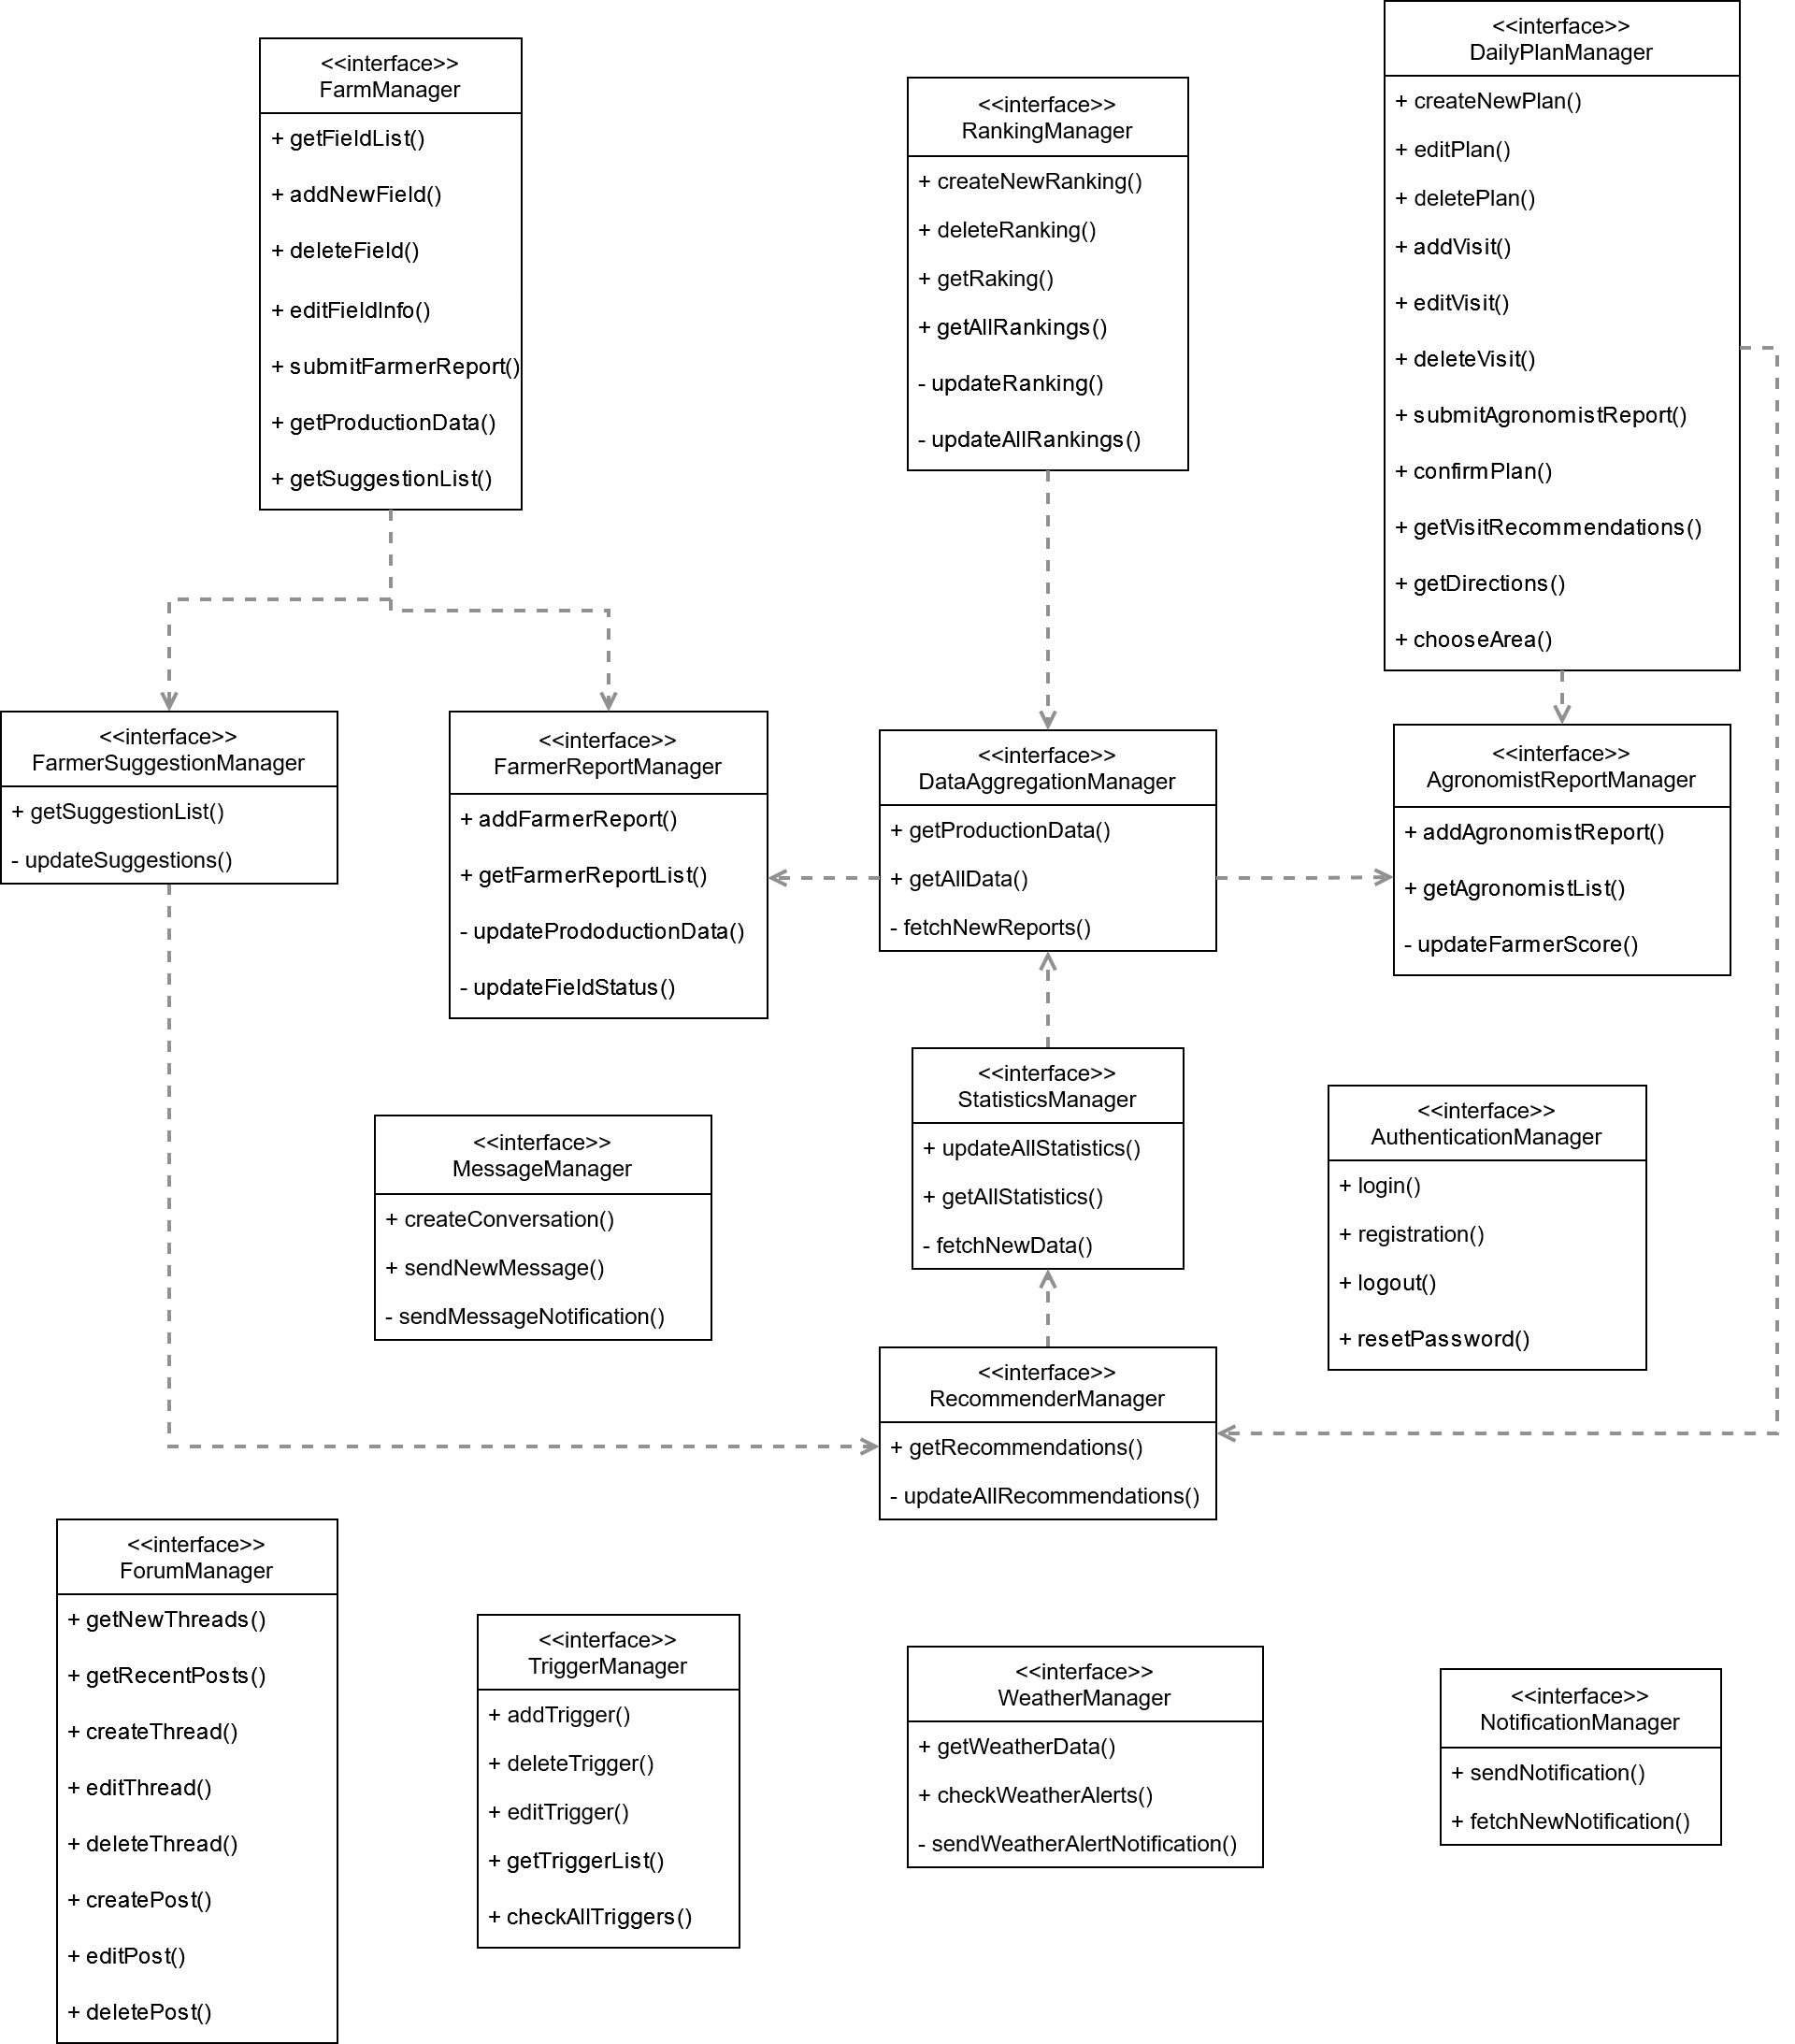
\includegraphics[width=\textwidth]{../images_diagrams/dd/component_interfaces_diagram.png}
\caption{Application Server Component Interfaces Diagram.}
\label{fig:componentInterface}
\end{figure}

\subsection{Selected Architectural Styles and Patterns}
Please explain which styles/patterns you used, why, and how
\subsection{Other Design Decisions}